\documentclass[11pt,a4paper]{report}%especifica o tipo de documento que tenciona escrever: carta, artigo, relatório... neste caso é um relatório
% [11pt,a4paper] Define o tamanho principal das letras do documento. caso não especifique uma delas, é assumido 10pt
% a4paper -- Define o tamanho do papel.

\usepackage[portuges]{babel}%Babel -- irá activar automaticamente as regras apropriadas de hifenização para a língua todo o
                                   %-- o texto gerado é automaticamente traduzido para Português.
                                   %  Por exemplo, “chapter” irá passar a “capítulo”, “table of contents” a “conteúdo”.
                                   % portuges -- específica para o Português.
\usepackage[utf8]{inputenc} % define o encoding usado texto fonte (input)--usual "utf8" ou "latin1

\usepackage{graphicx} %permite incluir graficos, tabelas, figuras
\usepackage{url} % para utilizar o comando \url{}
\usepackage{enumerate} %permite escolher, nas listas enumeradas, se os iems sao marcados com letras ou numeros-romanos em vez de numeracao normal

%\usepackage{apalike} % gerar biliografia no estilo 'named' (apalike)

\usepackage{color} % Para escrever em cores

\usepackage{multirow} %tabelas com multilinhas
\usepackage{array} %formatação especial de tabelas em array

\usepackage[pdftex]{hyperref} % transformar as referências internas do seu documento em hiper-ligações.

%Exemplos de fontes -- nao e vulgar mudar o tipo de fonte
%\usepackage{tgbonum} % Fonte de letra: TEX Gyre Bonum
%\usepackage{lmodern} % Fonte de letra: Latin Modern Sans Serif
%\usepackage{helvet}  % Fonte de letra: Helvetica
%\usepackage{charter} % Fonte de letra:Charter

\definecolor{saddlebrown}{rgb}{0.55, 0.27, 0.07} % para definir uma nova cor, neste caso 'saddlebrown'

\usepackage{listings}  % para utilizar blocos de texto verbatim no estilo 'listings'
%paramerização mais vulgar dos blocos LISTING - GENERAL
\lstset{
	basicstyle=\small, %o tamanho das fontes que são usadas para o código
	numbers=left, % onde colocar a numeração da linha
	numberstyle=\tiny, %o tamanho das fontes que são usadas para a numeração da linha
	numbersep=5pt, %distancia entre a numeração da linha e o codigo
	breaklines=true, %define quebra automática de linha
    frame=tB,  % caixa a volta do codigo
	mathescape=true, %habilita o modo matemático
	escapeinside={(*@}{@*)} % se escrever isto  aceita tudo o que esta dentro das marcas e nao altera
}
%
%\lstset{ %
%	language=Java,							% choose the language of the code
%	basicstyle=\ttfamily\footnotesize,		% the size of the fonts that are used for the code
%	keywordstyle=\bfseries,					% set the keyword style
%	%numbers=left,							% where to put the line-numbers
%	numberstyle=\scriptsize,				% the size of the fonts that are used for the line-numbers
%	stepnumber=2,							% the step between two line-numbers. If it's 1 each line
%											% will be numbered
%	numbersep=5pt,							% how far the line-numbers are from the code
%	backgroundcolor=\color{white},			% choose the background color. You must add \usepackage{color}
%	showspaces=false,						% show spaces adding particular underscores
%	showstringspaces=false,					% underline spaces within strings
%	showtabs=false,							% show tabs within strings adding particular underscores
%	frame=none,								% adds a frame around the code
%	%abovecaptionskip=-.8em,
%	%belowcaptionskip=.7em,
%	tabsize=2,								% sets default tabsize to 2 spaces
%	captionpos=b,							% sets the caption-position to bottom
%	breaklines=true,						% sets automatic line breaking
%	breakatwhitespace=false,				% sets if automatic breaks should only happen at whitespace
%	title=\lstname,							% show the filename of files included with \lstinputlisting;
%											% also try caption instead of title
%	escapeinside={\%*}{*)},					% if you want to add a comment within your code
%	morekeywords={*,...}					% if you want to add more keywords to the set
%}

\usepackage{xspace} % deteta se a seguir a palavra tem uma palavra ou um sinal de pontuaçao se tiver uma palavra da espaço, se for um sinal de pontuaçao nao da espaço

\parindent=0pt %espaço a deixar para fazer a  indentação da primeira linha após um parágrafo
\parskip=2pt % espaço entre o parágrafo e o texto anterior

\setlength{\oddsidemargin}{-1cm} %espaço entre o texto e a margem
\setlength{\textwidth}{18cm} %Comprimento do texto na pagina
\setlength{\headsep}{-1cm} %espaço entre o texto e o cabeçalho
\setlength{\textheight}{23cm} %altura do texto na pagina

% comando '\def' usado para definir abreviatura (macros)
% o primeiro argumento é o nome do novo comando e o segundo entre chavetas é o texto original, ou sequência de controle, para que expande
\def\darius{\textsf{Darius}\xspace}
\def\antlr{\texttt{AnTLR}\xspace}
\def\pe{\emph{Publicação Eletrónica}\xspace}
\def\titulo#1{\section{#1}}    %no corpo do documento usa-se na forma '\titulo{MEU TITULO}'
\def\super#1{{\em Supervisor: #1}\\ }
\def\area#1{{\em \'{A}rea: #1}\\[0.2cm]}
\def\resumo{\underline{Resumo}:\\ }

%\input{LPgeneralDefintions} %permite ler de um ficheiro de texto externo mais definições

\title{Processamento de Linguagens e Compiladores\\
       \textbf{Trabalho Prático 1}\\ Relatório de Desenvolvimento
       } %Titulo do documento
%\title{Um Exemplo de Artigo em \LaTeX}
\author{Miguel Gonçalves\\ a90416 \and João Nogueira\\ a87973
         \and Rui Baptista\\ a87989
       } %autores do documento
\date{\today} %data

\begin{document} % corpo do documento
\maketitle % apresentar titulo, autor e data

\begin{abstract}  % resumo do documento
O seguinte relatório documenta, justifica, analisa e expõe todas as decisões tomadas ao longo do Trabalho Prático realizado no âmbito da Unidade Curricular denominada Processamento de Linguagens e Compiladores no contexto do 3º ano do curso Licenciatura em Ciências da Computação.\\
O seguinte trabalho era um dos 5 que nos foi apresentados na Unidade Curricular, visto que somos o grupo 8,
usando a formula (NGr \% 7) + 1 verificamos que nos calhou o trabalho nº2. Este consistia em criar 4 programas Python para processar o ficheiro de texto "processos.txt"
com o intuito de calcular frequências de alguns elementos.\\
\end{abstract}

\tableofcontents % Insere a tabela de indice
%\listoffigures % Insere a tabela de indice figuras
%\listoftables % Insere a tabela de indice tabelas

\chapter{Introdução} \label{chap:intro} %referência cruzada
\titulo{Processador de Pessoas listadas nos Róis de Confessados}

Vamos agora enquadrar e contextualizar o trabalho.
É-nos dado um ficheiro onde se encontram vários dados, entre eles nomes, datas e relações familiares de várias pessoas, que estariam guardados no arquivo municipal de Braga.
Temos como intuito extrair, de forma objetiva, através de expressões regulares e outras estratégias dadas nas aulas, de forma a hipoteticamente ser possível analisar os dados em questão.
No capítulo 2 iremos fazer uma breve introdução ao enunciado, descrevendo assim os problemas que nos são propostos, além dos pensamentos iniciados antes de resolver os problemas.
No capítulo 3 explicaremos detalhadamente a solução para cada um dos problemas propostos, incluindo não só as expressões regulares, mas também os métodos com que estas são utilizadas de forma a extrair a informação necessária do ficheiro, decisões tomadas e ainda alguns testes realizados e resultados dos mesmos, de forma a comprovar a eficácia do nosso trabalho.



\chapter{Análise do problema} \label{chap:analiseEspecificacao} %capitulo e referencia cruzada
\section{Descrição informal do problema} \label{sec:descricaoProblema} %seccao e referencia cruzada

No enunciado é nos dado um ficheiro, neste caso o “processos.txt”, sobre o qual devemos desenvolver programas em Python de forma a resolver as seguintes questões :\\
\begin{enumerate}
a)	Calcular a frequência de processos por ano\\
\\
b)	Calcular a frequência de nomes\\
\\
c)	Calcular a frequência dos vários tipos de relação\\
\\
d)	Imprimir os 20 primeiros registos num novo ficheiro de output, em formato Json\\
\end{enumerate}

Vejamos agora um excerto do texto dado :
\begin{verbatim}
569::1867-05-23::Abel Alves Barroso::Antonio Alves Barroso::Maria Jose Alvares Barroso::
Bento Alvares Barroso,Tio Paterno. Proc.32057.
\end{verbatim}
É possível observar que toda a informação está condensada e misturada, havendo a necessidade de descobrir maneiras de identificar os vários tipos de informação pedida, sendo possível disponibilizá-la de acordo com cada uma das alíneas a cima referidas.\\
Desta forma, existe a necessidade de desenvolver estratégias e expressões regulares que se adequem a cada um dos problemas, desprezando a informação indesejada e mantendo apenas a que foi pedida.
Ao longo da resolução dos problemas, decidimos separar a informação em grupos convenientemente decididos, tendo em conta qual parte da informação é pedida por alínea, através das estratégias que serão mais à frente explicadas.

\newpage

\section{Estratégia inicial adoptada} \label{sec:estrategiaAdoptada}

Quando fomos confrontados com o enunciado, após a leitura do mesmo e do ficheiro dado, discutimos várias ideias sobre qual seria a melhor forma de abordar o problema em questão. Visto que queríamos calcular a frequência de processos por ano, deliberámos a forma correta de os identificar. \\
Concluímos então que existia um padrão, sendo este “número do processo :: data”. Através desta ideia, pretendemos adaptar a expressão regular e o código do programa de forma a identificar este padrão e guardar a sua frequência.\\
Após termos chegado à conclusão da existência de padrões, efetuámos o mesmo com o problema seguinte. Deparámo-nos com o padrão em que os nomes estariam sempre antecedidos por dois pontos, sendo assim o padrão predominante “::Nome Completo”. Em certas exceções é possível observar que existem nomes que se encontram da forma “.Nome Completo,”. Tal como anteriormente, após esta descoberta procedemos à tentativa de adaptação tanto do programa como da expressão regular de forma a que identificassem este padrão.\\
Para o problema dos vários tipos de relação, houve maior dificuldade em padronizar os dados existentes acerca dessas mesmas relações. As relações poderiam estar tanto no singular como no plural, algo importante a ter em consideração. Eventualmente concluímos que todas as relações, quer estejam no singular ou no plural, estariam compreendidas entre um ponto e uma vírgula, da forma “, Relação.”. Após esta conclusão, procedemos à escrita do código e respetiva expressão regular.

\newpage

\chapter{Soluções criadas}
Como referido, para melhor compreensão por parte do leitor, vamos falar das soluções criadas para cada alínea separadamente.
\section{Problema a}

\subsection{ER}

Começamos então por definir a nossa expressão regular que vai retirar todos os processos e as suas respetivas datas.\\
Como sabemos que os processos e o ano são da forma, por exemplo, "575::1894" criamos a seguinte ER:

\begin{verbatim}
ER = ([0-9]+)::([0-9]{4})
\end{verbatim}

Ou seja, queremos procurar todos os numeros que estão antes de "::" que são o numero do processo e depois 4 numeros de 0 a 9, que será a data.\\

\subsection{Algoritmo}

Para começar a resolver este problema, primeiramente damos open ao ficheiro de texto "processos.txt":

\begin{verbatim}
f = open("processos.txt")
linhas = f.readlines()
\end{verbatim}

Após isso, vamos iterar por cada linha do texto e usando a nossa ER, retirar os processos e os anos:

\begin{verbatim}
for i in linhas:
    new_text = re.search(r'([0-9]{3})::([0-9]{4})', i)
\end{verbatim}

Aqui usamos o search e não o findall, porque como estamos a procurar em cada linha, só vamos encontrar uma ocorrência do processo e do ano
\\
\\
\\
\\
\\
Depois guardamos o tuplo (ano,processo) num dicionário como key e criamos um contador para ser possivel calcular a frequência:

\begin{verbatim}
datas = {}

    if new_text:
        data = new_text.group(2)
        processo = new_text.group(1)
        if (data,processo) not in datas: 
            datas[(data,processo)] = 1 
        else: 
            datas[((data,processo))] += 1 
\end{verbatim}

No fim damos então print ao nosso dicionário com a seguinte estrutura:

\begin{verbatim}
for (a,b) in datas: 
    print("No ano " + str(a) + ", o processo " + str(b) + " aconteceu " + str(datas[a,b]) + " vezes")
\end{verbatim}
\subsection{Exemplo de funcionamento}

Para mostrar o bom funcionamento do nosso programa vamos dar como input, por exemplo, as seguintes linhas de texto:

\begin{verbatim}
575::1894-11-08::Aarao Pereira Silva::Antonio Pereira Silva::Francisca Campos Silva::::
582::1909-05-12::Abel Almeida::Antonio Manuel Almeida::Teresa Maria Sousa::::
575::1894-04-30::Abelardo Jose Cerqueira Araujo::Jose Maria Araujo::Leopoldina Cerqueira Ribeiro Araujo::::
18::1691-05-26::Adriano Azevedo::Gabriel Azevedo::Jeronima Andrade Veloso::::
\end{verbatim}

Executando o programa recebemos o seguinte output:


\begin{center}
    \includegraphics[width=.4\textwidth]{aex.png}
    \\
    \caption{Figura 1. Exemplo do programa a)}
\end{center}

Logo verificamos que o nosso programa está a funcionar corretamente.


\newpage
\section{Problema b}

\subsection{ER}

Como pretendemos reconhecer todos os nomes, criamos a seguinte expressão regular:

\begin{verbatim}
ER = ([a-zA-Z]+[ ]?)+
\end{verbatim}

\subsection{Algoritmo}

Observámos que todos os nomes são antecedidos por “::”, como por exemplo “::Adriano Duarte”. Sendo assim, a primeira coisa que fizemos foi um re.split
onde o separador é "::". 

\begin{verbatim}
for linha in linhas: 
    lista = re.split(r'::',linha)
\end{verbatim}

Desta forma ao receber uma linha de texto, por exemplo, "575::1894-11-08::Aarao Pereira Silva"  vamos transformar essa linha na lista
"575", "894-11-08", "Aarao Pereira Silva", desta forma a nossa ER consegue apanhar todos os nomes.

\begin{verbatim}
for linha in linhas: 
    lista = re.split(r'::',linha)
    for elemento in lista: 
        new_text = re.search(r'([a-zA-Z]+[ ]?)+',elemento)
\end{verbatim}

Seguidamente guardamos então os nomes num dicionário e criamos um contador para calcular a frequência de cada nome.

\begin{verbatim}
relacao = {}

        if new_text: 
            texto = new_text.group() 
            if texto not in relacao: 
                relacao[texto] = 1 
            else: 
                relacao[texto] += 1 
\end{verbatim}

No fim damos print aos nomes guardados no dicionário e o respetivo contador

\begin{verbatim}
for rela in relacao: 
    print ("Nome: " + rela + ": " + str(relacao[rela]))
\end{verbatim}

\newpage

\subsection{Exemplo de funcionamento}

Para mostrar o bom funcionamento do nosso programa vamos dar como input, por exemplo, as seguintes linhas de texto:

\begin{verbatim}
579::1904-05-27::Abel Gomes Abreu Reis::Antonio Gomes Abreu::Ana Sequeira Reis::::
579::1904-05-21::Abel Marques Reis::Jose Joaquim Marques Reis::Bernardina Dantas::::
581::1908-05-20::Abilio Augusto Magalhaes::::Maria Jesus Magalhaes::::
581::1908-05-20::Abilio Augusto Magalhaes::::Maria Jesus Magalhaes::::
\end{verbatim}

Executando o programa recebemos o seguinte output:

\begin{center}
    \includegraphics[width=.4\textwidth]{bex.png}
    \\
    \caption{Figura 2. Exemplo do programa b)}
\end{center}

Como podemos verificar, o programa lê corretamente todos os nomes e a sua respetiva frequência.

\section{Problema c}

\subsection{ER}

Pretendemos identificar e calcular a frequência dos vários tipos de relações familiares.\\
Observámos que todas as relações seriam escritas após nomes, sendo antecedidas por uma vírgula e após as mesmas estaria um ponto. 
Utilizámos o findall para encontrar todas as ocorrências dos vários tipos de relações, em conjunto com a seguinte expressão regular:

\begin{verbatim}
ER = (?i)(\birma[o]?|\bsobrinh[oa]|\bavo|\bti[oa]|\bprim[oa]|\bpai|\bfilh[oa]|\bmae)
([ ]+?[a-zA-Z]+[.,])?
\end{verbatim}

Incluímos todos os graus de parentesco identificados na ER, tendo em conta que estes poderiam estar no masculino ou feminino, e que poderiam ser seguidores de um semi grau de parentesco, por exemplo Sobrinho Neto.



\subsection{Algoritmo}

Começamos então por iterar por cada linha do ficheiro de texto e fazer um re.split. Depois para cada elemento nessa nova lista que o split devolve aplicamos a nossa ER.

\begin{verbatim}
for linha in linhas: 
    lista = re.split(r'::',linha)
    for elemento in lista: 
        new_text = re.findall(r'(?i)(\birma[o]?|\bsobrinh[oa]|\bavo|\bti[oa]|\bprim[oa]|
        \bpai|\bfilh[oa]|\bmae)([ ]+?[a-zA-Z]+[.,])?',elemento)

\end{verbatim}

\newpage

Tivemos ainda em conta que algumas destas relações poderiam ser apresentadas no plural, adequando assim o nosso código de forma a que fossem também incluídas na contagem dessa mesma relação, mas no singular.

\begin{verbatim}
for palavra in a:
    por = palavra
    aux = list(por)
    if aux[len(aux)-1] == 's': 
       del(aux[len(aux)-1])
    aux[0] = aux[0].upper()
    por = ''.join(aux[i] for i in range(len(aux)))
\end{verbatim}

Por fim, de forma a ser possível calcular a frequência, criamos um contador.

\begin{verbatim}
if por not in relacao: 
    relacao[por] = 1 
else: 
    elacao[por] += 1 
\end{verbatim}

\subsection{Exemplo de funcionamento}


Para mostrar o bom funcionamento do nosso programa vamos dar como input, por exemplo, as seguintes linhas de texto:

\begin{verbatim}
30::1703-08-09::Adriano Duarte::Doc.danificado.  Domingos Duarte,Irmao. Proc.23448.::
384::1780-01-22::Agostinho Fernandes,Tio Materno.  Joao Fernandes,Tio Paterno.::
254::1730-11-20::Mariana Pinto,Solteira::Doc.danificado.  Inacio Castro Rocha,Pai. Proc.1628.::
\end{verbatim}

Como podemos ver, temos 1 ocorrência da relação Irmao, 2 ocorrências de Tio e 1 de Pai, vamos então executar o programa para ver se isto se verifica:

\begin{center}
    \includegraphics[width=.3\textwidth]{cex.png}
    \\
    \caption{Figura 2. Exemplo do programa c)}
\end{center}

Como podemos verificar no output do o programa, este identifica corretamente os vários tipos de relações.

\newpage

Executando de novo a nossa solução, mas agora sendo o processos.txt o input, obetemos o seguinte output:

\begin{center}
    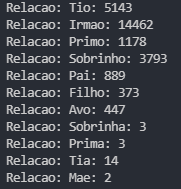
\includegraphics[width=.3\textwidth]{c.png}
    \\
    \caption{Figura 3. Output do programa c) com processos.txt como input}
\end{center}

Para verificar a veracidade do output, vamos confirmar no ficheiro de texto se os valores estão de facto corretos.
\begin{center}
    
\includegraphics[width=.4\textwidth]{tio.png}
    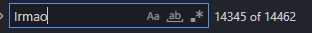
\includegraphics[width=.4\textwidth]{irmao.png}
    \\
    \caption{Figura 4. Confirmação dos valores}
\end{center}

Como podemos verificar, os valores para as relações estão corretos.

\newpage

\section{Problema d}

\subsection{ER}

Como esta alínea pedia apenas para imprimir os primeiros 20 registos em formato Json, não foi preciso definir uma ER.

\subsection{Algoritmo}

Primeiramente como o problema pede para imprimir os primeiros 20 registos, vamos abrir o nosso ficheiro de texto, mas ler só as primeiras 20 linhas.

\begin{verbatim}
N=20
with open("processos.txt", "r") as fileoriginal:
    fileN = [next(fileoriginal) for x in range(N)]
\end{verbatim}

De seguida, voltamos a usar a tática de fazer re.split a cada linha do nosso texto:

\begin{verbatim}
for v in fileN: 
    lista = re.split(r'::|[ ]+[ ]+',v)
\end{verbatim}

Depois vamos adicionar cada linha a um dicionário e no fim dessa linha passamos esse dicionário para uma lista
\begin{verbatim}
dic = {}
listadics = []

for elemento in lista: 
        if elemento != '\n' and elemento != '': 
            if contador == 0: 
                dic["numero processo"] = elemento
            elif contador == 1: 
                dic["data"] = elemento
            elif contador >= 2: 
                dic["nome(s)" + str(nome)] = elemento
                nome += 1
            contador += 1
    listadics.append(dic)
\end{verbatim}

Por fim, damos print ao nosso dicionário em formato JSON usando o seguinte comando:

\begin{verbatim}
with open("json.json", 'w') as file:
    file.write((json.dumps(listadics, indent=4, sort_keys= False)))
\end{verbatim}


\subsection{Exemplo de funcionamento}
Ao receber, por exemplo, as seguintes linhas de texto:

\begin{verbatim}
575::1894-11-08::Aarao Pereira Silva::Antonio Pereira Silva::Francisca Campos Silva::::
582::1909-05-12::Abel Almeida::Antonio Manuel Almeida::Teresa Maria Sousa::::
\end{verbatim}

O nosso programa tem o seguinte output:
\begin{center}
    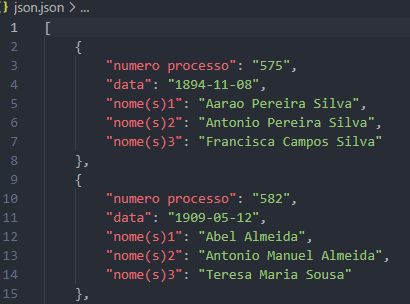
\includegraphics[width=.4\textwidth]{d.png}
    \\
    \caption{Figura 5. Exemplo do programa d) }
\end{center}

Como podemos verificar, imprime corretamente as duas linhas em formato Json.\\
\\
Para verificar que o output para as 20 linhas que é pedido no enunciado está de facto correto, usamos o site \textbf{jsonformatter.curiousconcept.com}, onde passamos o ficheiro Json que o nosso programa gera e verificamos se tá correto ou não:

\begin{center}
    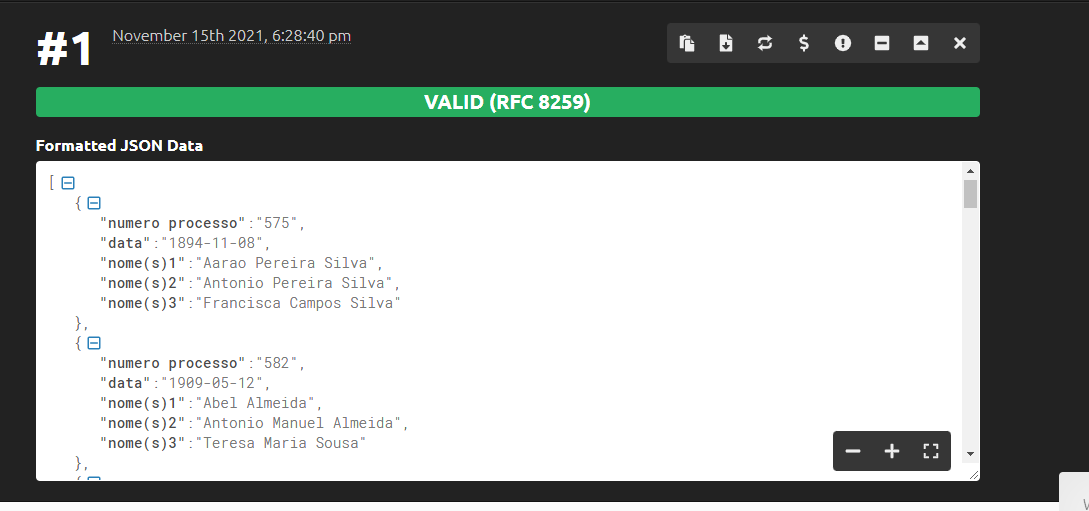
\includegraphics[width=.7\textwidth]{json.png}
    \\
    \caption{Figura 6. Confirmação do ficheiro Json }
\end{center}

O site validou o ficheiro Json gerado pelo nosso programa para as primeiras 20 linhas, confirmando assim o seu bom funcionamento.

%\chapter{Codificação e Testes}
%\section{Alternativas, Decisões e Problemas de Implementação}
%\section{Testes realizados e Resultados}
%Mostram-se a seguir alguns testes feitos (valores introduzidos) e
%os respectivos resultados obtidos:
%\VerbatimInput{teste1.txt}

\chapter{Conclusão} \label{concl}
Este trabalho revelou-se bastante útil para a consolidação de vários temas, como a utilização de expressões regulares e ferramentas como o search e findall.
\\
Permitiu-nos ainda perceber as aplicações reais dos conceitos, mostrando na prática o quão útil realmente são essas ERs e ferramentas. Embora tenha havido algumas dificuldades, na nossa opinião o grupo esteve à altura do desafio. Trabalhámos e aplicámos as ferramentas de forma que nos fossem úteis, atingindo com clareza o objetivo do trabalho, sendo este a filtragem do texto proposto e o respetivo cálculo das frequências.
\\
Estamos bastante satisfeitos com o resultado final, percebendo que a matéria dada foi absorvida corretamente, tendo este trabalho um papel muito importante nesse aspeto.
\\
Por fim, ficamos com várias ferramentas à nossa disposição para problemas e desafios futuros, sabendo que estas são bastante úteis, práticas e eficazes.

\appendix % apendice

\chapter{Código da alínea a)}
%\section{Código da alínea a)}

\begin{lstlisting}
import re

f = open("processos.txt")
linhas = f.readlines()
datas = {}

for i in linhas:
    new_text = re.search(r'([0-9]+)::([0-9]{4})', i)
    if new_text:
        data = new_text.group(2)
        processo = new_text.group(1)
        if (data,processo) not in datas: 
            datas[(data,processo)] = 1 
        else: 
            datas[((data,processo))] += 1 
f.close()
for (a,b) in datas: 
    print("No ano " + str(a) + ", o processo " + str(b) + " aconteceu " + str(datas[a,b]) + " vezes")

\end{lstlisting}

\newpage

\chapter{Código da alínea b)}
%\section{Código da alínea b)}

\begin{lstlisting}
import re

f = open("processos.txt")
linhas = f.readlines()
relacao = {}

for linha in linhas: 
    lista = re.split(r'::',linha)
    for elemento in lista: 
        new_text = re.search(r'([a-zA-Z]+[ ]?)+',elemento)
        if new_text: 
            texto = new_text.group() 
            if texto not in relacao: 
                relacao[texto] = 1 
            else: 
                relacao[texto] += 1 

for rela in relacao: 
    print ("Nome: " + rela + ": " + str(relacao[rela]))
\end{lstlisting}

\newpage

\chapter{Código da alínea c)}
%\section{Código da alínea c)}


\begin{lstlisting}
import re

f = open("processos.txt")
linhas = f.readlines()
relacao = {}

for linha in linhas: 
    lista = re.split(r'::',linha)
    for elemento in lista: 
        new_text = re.findall(r'(?i)(\birma[o]?|\bsobrinh[oa]|\bavo|\bti[oa]|\bprim[oa]|\bpai|\bfilh[oa]|\bmae)([ ]+?[a-zA-Z]+[.,])?',elemento)
        if new_text:
            a = []
            for k in range(len(new_text)): 
                a.append(new_text[k][0])

            for palavra in a:
                por = palavra
                aux = list(por)
                if aux[len(aux)-1] == 's': 
                    del(aux[len(aux)-1])
                aux[0] = aux[0].upper()
                por = ''.join(aux[i] for i in range(len(aux)))


                if por not in relacao: 
                    relacao[por] = 1 
                else: 
                    relacao[por] += 1 
for rela in relacao: 
    print ("Relacao: " + rela + ": " + str(relacao[rela]))
\end{lstlisting}

\newpage

\chapter{Código da alínea d)}
%\section{Código da alínea d)}

\begin{lstlisting}
import re 
import json 

listadics = []
N=20
with open("processos.txt", "r") as fileoriginal:
    fileN = [next(fileoriginal) for x in range(N)]

for v in fileN: 
    lista = re.split(r'::|[ ]+[ ]+',v)
    dic = {}
    contador = 0 
    nome = 1 
    linha = 0 
    for elemento in lista: 
        if elemento != '\n' and elemento != '': 
            if contador == 0: 
                dic["numero processo"] = elemento
            elif contador == 1: 
                dic["data"] = elemento
            elif contador >= 2: 
                dic["nome(s)" + str(nome)] = elemento
                nome += 1
            contador += 1
    listadics.append(dic)
    
with open("json.json", 'w') as file:
    file.write((json.dumps(listadics, indent=4, sort_keys= False)))
\end{lstlisting}


%-- Fim do documento -- inserção das referencias bibliográficas

%\bibliographystyle{plain} % [1] Numérico pela ordem de citação ou ordem alfabetica
%\bibliographystyle{alpha} % [Hen18] abreviação do apelido e data da publicação
%\bibliographystyle{apalike} % (Araujo, 2018) apelido e data da publicação
                             % --para usar este estilo descomente no inicio o comando \usepackage{apalike}

%\bibliography{bibLayout} %input do ficheiro de referencias bibliograficas

\end{document} 
